\subsection{複素積分}
	$\gamma$を$[\alpha,\beta]$から$\C$への関数で,右連続かつ有界変動であるとする.
	このとき$\gamma$を$[\alpha,\beta]$上の{\bf 路}\index{ろ@路}
	{\bf (contour)}と呼ぶ.$\gamma$から作る複素Stieltjes測度を
	\begin{align}
		\mu_\gamma
	\end{align}
	とする.$\gamma$は$[\alpha,\beta]$から$\C$への可測関数であるから
	\begin{align}
		\tilde{\mu}_\gamma(A) \defeq \mu_\gamma\left( \gamma^{-1}(A) \right),
		\quad (A \in \borel{\C})
	\end{align}
	で定める$\tilde{\mu}_\gamma$は$(\C,\borel{\C})$上の複素測度となり,このとき
	$\Omega$上の関数$f$を$|\tilde{\mu}_\gamma|$に関する可積分関数とすれば
	\begin{align}
		\int_\Omega f\ d\tilde{\mu}_\gamma = \int_{[\alpha,\beta]} f(\gamma)\ d\mu_\gamma
	\end{align}
	が成立する.特に$\gamma$が$[\alpha,\beta]$上で絶対連続なら,
	$\lambda$を一次元Lebesgue測度とすれば
	\begin{align}
		\mu_\gamma(E) = \int_E \gamma'\ d\lambda,
		\quad (\forall E \in \borel{[\alpha,\beta]})
	\end{align}
	となるので
	\begin{align}
		\int_{[\alpha,\beta]} f(\gamma)\ d\mu_\gamma = \int_{[\alpha,\beta]} f(\gamma) \cdot \gamma'\ d\lambda
	\end{align}
	が成立する.
	$\gamma$に関する$f$の複素(線)積分を
	\begin{align}
		\int_\gamma f \defeq \int_\Omega f\ d\tilde{\mu}_\gamma
	\end{align}
	で定義する.
	
	$\gamma$は$[\alpha,\beta]$上の写像であったが,$\gamma$に関する線積分はパラメータ変項で不変であることを示す.
	\begin{align}
		\varphi:[\alpha_1,\beta_1] \longrightarrow [\alpha,\beta]
	\end{align}
	で
	\begin{align}
		x \in [\alpha_1,\beta_1] \Longrightarrow \varphi(x) = \alpha + \frac{\beta-\alpha}{\beta_1-\alpha_1}(x-\alpha_1)
	\end{align}
	なる$\varphi$により
	\begin{align}
		\gamma_1 \coloneqq \gamma \circ \varphi
	\end{align}
	と定めれば,
	\begin{align}
		\int_\gamma f = \int_{\gamma_1} f
	\end{align}
	が成立する.これは
	\begin{align}
		\tilde{\mu}_\gamma = \tilde{\mu}_{\gamma_1}
	\end{align}
	が成り立つことを示せば良いが,
	\begin{align}
		\tilde{\mu}_\gamma = \mu_\gamma \circ \gamma^{-1},
		\quad \tilde{\mu}_{\gamma_1} = \mu_{\gamma_1} \circ \varphi^{-1} \circ \gamma^{-1} 
	\end{align}
	であり,$\gamma$は$[\alpha,\beta]$上のBorel可測関数であるから,
	\begin{align}
		\forall E \in \borel{[\alpha,\beta]}\, 
		\left(\, \mu_{\gamma_1} \circ \varphi^{-1}(E) = \mu_\gamma(E)\, \right)
	\end{align}
	を示せば良い.$E$が$(s,t]$なる形の場合は
	\begin{align}
		\mu_{\gamma_1} \circ \varphi^{-1}((s,t])
		&= \mu_{\gamma_1} \left(\left(\varphi^{-1}(s),\varphi^{-1}(t)\right]\right) \\
		&= \gamma_1\left( \varphi^{-1}(t) \right) - \gamma_1\left( \varphi^{-1}(s) \right) \\
		&= \gamma(t) - \gamma(s) \\
		&= \mu_\gamma((s,t])
	\end{align}
	が成り立つ.$E = \{\alpha\}$なら
	\begin{align}
		\mu_{\gamma_1} \circ \varphi^{-1}(\{\alpha\})
		= \mu_{\gamma_1}(\{\alpha_1\})
		= 0
		= \mu_\gamma(\{\alpha\})
	\end{align}
	が成り立つ.一致の定理より
	\begin{align}
		\mu_{\gamma_1} \circ \varphi^{-1} = \mu_\gamma
	\end{align}
	となる.
	
	次に逆向きの路に関する積分を考える.$\gamma$が連続であるとき,
	\begin{align}
		\gamma_2 : [\alpha,\beta] \longrightarrow \C
	\end{align}
	で
	\begin{align}
		t \in [\alpha, \beta] \Longrightarrow \gamma_2(t) = \gamma(\alpha + \beta - t) 
	\end{align}
	を満たす$\gamma_2$は有界変動かつ連続となるので,複素Stieltjes測度を構成できる.
	$\gamma_2$を$\gamma$の{\bf 逆路}\index{ぎゃくろ@逆路}{\bf (inverse contour)}と呼ぶ.
	このとき
	\begin{align}
		\int_{\gamma_2} f = - \int_\gamma f
	\end{align}
	が成立する.これは
	\begin{align}
		\tilde{\mu}_{\gamma_2} = - \tilde{\mu}_\gamma 
	\end{align}
	を示せば良いが,
	\begin{align}
		\psi(t) = \alpha + \beta - t
	\end{align}
	なる$\psi:[\alpha,\beta] \longrightarrow [\alpha,\beta]$を定めれば
	\begin{align}
		\mu_{\gamma_2} \gamma_2^{-1} = \mu_{\gamma_2} \circ \psi^{-1} \circ \gamma^{-1}
	\end{align}
	となるので
	\begin{align}
		\forall E \in \borel{[\alpha,\beta]}\,
		\left(\, \mu_{\gamma_2}(\psi^{-1} \ast E) = -\mu_\gamma(E)\, \right)
	\end{align}
	を示せば十分である.$E$が$(s,t)$なる形の場合
	\begin{align}
		\mu_{\gamma_2}\left(\psi^{-1} \ast (s,t)\right)
		&= \mu_{\gamma_2}\left( \left( \psi^{-1}(t),\psi^{-1}(s) \right) \right) \\
		&= \gamma_2\left(\psi^{-1}(s)\right) - \gamma_2\left(\psi^{-1}(t)\right) \\
		&= \gamma(s) - \gamma(t) \\
		&= -\mu_\gamma((s,t))
	\end{align}
	が成立する.$\mu_\gamma$も$\mu_{\gamma_2}$も一点の測度は$0$であるから
	\begin{align}
		\mu_{\gamma_2} \circ \psi^{-1} = -\mu_\gamma
	\end{align}
	が従う.
	
	\begin{screen}
		\begin{thm}[正則関数に対する微積分学の基本定理]
			$f$を$H(\Omega)$の要素とし,$f'$が連続であるとし,$\gamma$を$[\alpha,\beta]$から$\Omega$への絶対連続な路とする.このとき
			\begin{align}
				\int_{\gamma} f' = f(\gamma(\beta)) - f(\gamma(\alpha))
			\end{align}
			が成立する.特に$\gamma$が閉路なら積分値は$0$である.
		\end{thm}
	\end{screen}
	
	\begin{prf}
		微積分学の基本定理より
		\begin{align}
			\int_{\gamma} f'
			= \int_{[\alpha,\beta]} f'(\gamma(t)) \cdot \gamma'(t)\ dt
			= f(\gamma(\beta)) - f(\gamma(\alpha))
		\end{align}
		となる.
		\QED
	\end{prf}
	
	$a$と$b$と$c$を複素数とすると,
	\begin{align}
		\Delta \defeq \Set{z}{\exists s,t \in [0,1]\, 
		\left(\, z = (1-t) \cdot a 
		+ t \cdot (1-s) \cdot b 
		+ t \cdot s \cdot c\, \right)}
	\end{align}
	により定める集合$\Delta$は,イメージとしては$a,b,c$によって囲まれる三角領域
	
	\begin{center}
	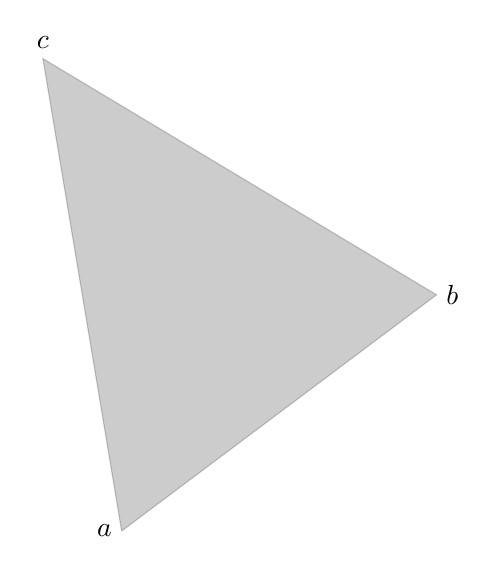
\begin{tikzpicture}
		\filldraw[opacity=0.2] (0,0)--(4,3)--(-1,6)--(0,0);
		\node[anchor=east] at (0,0) {$a$};
		\node[anchor=west] at (4,3) {$b$};
		\node[anchor=south] at (-1,6) {$c$};
	\end{tikzpicture}
	\end{center}
	
	を表す.